% Created by tikzDevice version 0.12.3.1 on 2023-05-29 17:59:51
% !TEX encoding = UTF-8 Unicode
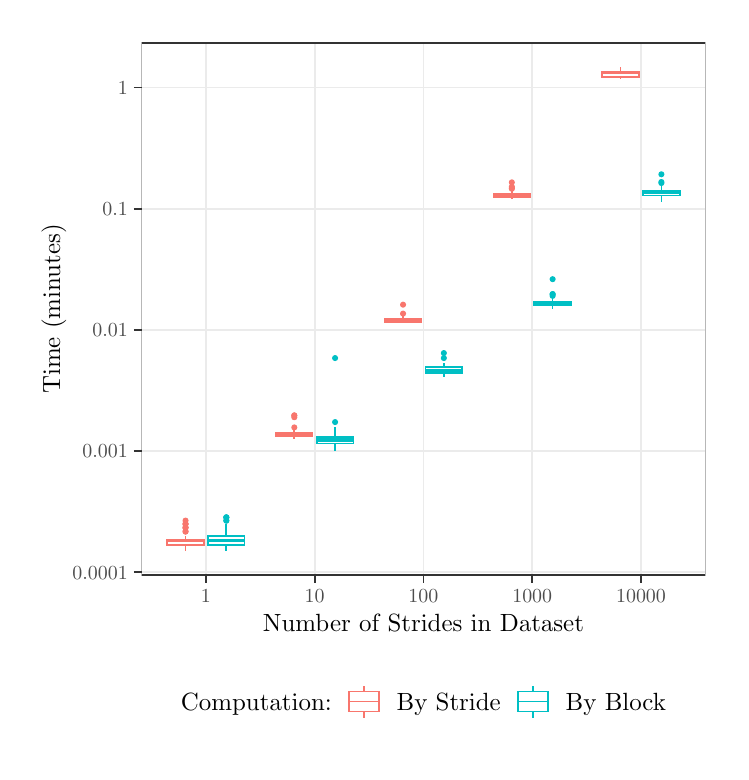
\begin{tikzpicture}[x=1pt,y=1pt]
\definecolor{fillColor}{RGB}{255,255,255}
\path[use as bounding box,fill=fillColor,fill opacity=0.00] (0,0) rectangle (250.38,261.76);
\begin{scope}
\path[clip] (  0.00,  0.00) rectangle (250.38,261.76);
\definecolor{drawColor}{RGB}{255,255,255}
\definecolor{fillColor}{RGB}{255,255,255}

\path[draw=drawColor,line width= 0.6pt,line join=round,line cap=round,fill=fillColor] ( -0.00, -0.00) rectangle (250.38,261.76);
\end{scope}
\begin{scope}
\path[clip] ( 41.14, 63.96) rectangle (244.88,256.26);
\definecolor{fillColor}{RGB}{255,255,255}

\path[fill=fillColor] ( 41.14, 63.96) rectangle (244.88,256.26);
\definecolor{drawColor}{gray}{0.92}

\path[draw=drawColor,line width= 0.6pt,line join=round] ( 41.14, 64.99) --
	(244.88, 64.99);

\path[draw=drawColor,line width= 0.6pt,line join=round] ( 41.14,108.78) --
	(244.88,108.78);

\path[draw=drawColor,line width= 0.6pt,line join=round] ( 41.14,152.56) --
	(244.88,152.56);

\path[draw=drawColor,line width= 0.6pt,line join=round] ( 41.14,196.35) --
	(244.88,196.35);

\path[draw=drawColor,line width= 0.6pt,line join=round] ( 41.14,240.14) --
	(244.88,240.14);

\path[draw=drawColor,line width= 0.6pt,line join=round] ( 64.41, 63.96) --
	( 64.41,256.26);

\path[draw=drawColor,line width= 0.6pt,line join=round] (103.71, 63.96) --
	(103.71,256.26);

\path[draw=drawColor,line width= 0.6pt,line join=round] (143.01, 63.96) --
	(143.01,256.26);

\path[draw=drawColor,line width= 0.6pt,line join=round] (182.32, 63.96) --
	(182.32,256.26);

\path[draw=drawColor,line width= 0.6pt,line join=round] (221.62, 63.96) --
	(221.62,256.26);
\definecolor{drawColor}{RGB}{248,118,109}
\definecolor{fillColor}{RGB}{248,118,109}

\path[draw=drawColor,line width= 0.4pt,line join=round,line cap=round,fill=fillColor] ( 57.04, 81.10) circle (  0.89);

\path[draw=drawColor,line width= 0.4pt,line join=round,line cap=round,fill=fillColor] ( 57.04, 81.10) circle (  0.89);

\path[draw=drawColor,line width= 0.4pt,line join=round,line cap=round,fill=fillColor] ( 57.04, 79.69) circle (  0.89);

\path[draw=drawColor,line width= 0.4pt,line join=round,line cap=round,fill=fillColor] ( 57.04, 82.42) circle (  0.89);

\path[draw=drawColor,line width= 0.4pt,line join=round,line cap=round,fill=fillColor] ( 57.04, 83.64) circle (  0.89);

\path[draw=drawColor,line width= 0.4pt,line join=round,line cap=round,fill=fillColor] ( 57.04, 82.42) circle (  0.89);

\path[draw=drawColor,line width= 0.4pt,line join=round,line cap=round,fill=fillColor] ( 57.04, 82.42) circle (  0.89);

\path[draw=drawColor,line width= 0.4pt,line join=round,line cap=round,fill=fillColor] ( 57.04, 79.69) circle (  0.89);

\path[draw=drawColor,line width= 0.4pt,line join=round,line cap=round,fill=fillColor] ( 57.04, 81.10) circle (  0.89);

\path[draw=drawColor,line width= 0.6pt,line join=round] ( 57.04, 76.52) -- ( 57.04, 78.17);

\path[draw=drawColor,line width= 0.6pt,line join=round] ( 57.04, 74.71) -- ( 57.04, 72.70);
\definecolor{fillColor}{RGB}{255,255,255}

\path[draw=drawColor,line width= 0.6pt,fill=fillColor] ( 50.40, 76.52) --
	( 50.40, 74.71) --
	( 63.67, 74.71) --
	( 63.67, 76.52) --
	( 50.40, 76.52) --
	cycle;

\path[draw=drawColor,line width= 1.1pt] ( 50.40, 76.52) -- ( 63.67, 76.52);
\definecolor{fillColor}{RGB}{248,118,109}

\path[draw=drawColor,line width= 0.4pt,line join=round,line cap=round,fill=fillColor] ( 96.34,121.64) circle (  0.89);

\path[draw=drawColor,line width= 0.4pt,line join=round,line cap=round,fill=fillColor] ( 96.34,121.64) circle (  0.89);

\path[draw=drawColor,line width= 0.4pt,line join=round,line cap=round,fill=fillColor] ( 96.34,117.31) circle (  0.89);

\path[draw=drawColor,line width= 0.4pt,line join=round,line cap=round,fill=fillColor] ( 96.34,120.98) circle (  0.89);

\path[draw=drawColor,line width= 0.6pt,line join=round] ( 96.34,115.34) -- ( 96.34,116.28);

\path[draw=drawColor,line width= 0.6pt,line join=round] ( 96.34,114.07) -- ( 96.34,113.27);
\definecolor{fillColor}{RGB}{255,255,255}

\path[draw=drawColor,line width= 0.6pt,fill=fillColor] ( 89.71,115.34) --
	( 89.71,114.07) --
	(102.97,114.07) --
	(102.97,115.34) --
	( 89.71,115.34) --
	cycle;

\path[draw=drawColor,line width= 1.1pt] ( 89.71,114.72) -- (102.97,114.72);
\definecolor{fillColor}{RGB}{248,118,109}

\path[draw=drawColor,line width= 0.4pt,line join=round,line cap=round,fill=fillColor] (135.64,158.43) circle (  0.89);

\path[draw=drawColor,line width= 0.4pt,line join=round,line cap=round,fill=fillColor] (135.64,161.66) circle (  0.89);

\path[draw=drawColor,line width= 0.6pt,line join=round] (135.64,156.39) -- (135.64,157.75);

\path[draw=drawColor,line width= 0.6pt,line join=round] (135.64,155.31) -- (135.64,154.94);
\definecolor{fillColor}{RGB}{255,255,255}

\path[draw=drawColor,line width= 0.6pt,fill=fillColor] (129.01,156.39) --
	(129.01,155.31) --
	(142.28,155.31) --
	(142.28,156.39) --
	(129.01,156.39) --
	cycle;

\path[draw=drawColor,line width= 1.1pt] (129.01,155.66) -- (142.28,155.66);
\definecolor{fillColor}{RGB}{248,118,109}

\path[draw=drawColor,line width= 0.4pt,line join=round,line cap=round,fill=fillColor] (174.95,203.81) circle (  0.89);

\path[draw=drawColor,line width= 0.4pt,line join=round,line cap=round,fill=fillColor] (174.95,205.86) circle (  0.89);

\path[draw=drawColor,line width= 0.4pt,line join=round,line cap=round,fill=fillColor] (174.95,203.55) circle (  0.89);

\path[draw=drawColor,line width= 0.4pt,line join=round,line cap=round,fill=fillColor] (174.95,204.31) circle (  0.89);

\path[draw=drawColor,line width= 0.6pt,line join=round] (174.95,201.80) -- (174.95,203.48);

\path[draw=drawColor,line width= 0.6pt,line join=round] (174.95,200.66) -- (174.95,199.93);
\definecolor{fillColor}{RGB}{255,255,255}

\path[draw=drawColor,line width= 0.6pt,fill=fillColor] (168.32,201.80) --
	(168.32,200.66) --
	(181.58,200.66) --
	(181.58,201.80) --
	(168.32,201.80) --
	cycle;

\path[draw=drawColor,line width= 1.1pt] (168.32,201.20) -- (181.58,201.20);

\path[draw=drawColor,line width= 0.6pt,line join=round] (214.25,245.81) -- (214.25,247.52);

\path[draw=drawColor,line width= 0.6pt,line join=round] (214.25,243.96) -- (214.25,243.23);

\path[draw=drawColor,line width= 0.6pt,fill=fillColor] (207.62,245.81) --
	(207.62,243.96) --
	(220.88,243.96) --
	(220.88,245.81) --
	(207.62,245.81) --
	cycle;

\path[draw=drawColor,line width= 1.1pt] (207.62,245.62) -- (220.88,245.62);
\definecolor{drawColor}{RGB}{0,191,196}
\definecolor{fillColor}{RGB}{0,191,196}

\path[draw=drawColor,line width= 0.4pt,line join=round,line cap=round,fill=fillColor] ( 71.78, 84.80) circle (  0.89);

\path[draw=drawColor,line width= 0.4pt,line join=round,line cap=round,fill=fillColor] ( 71.78, 83.64) circle (  0.89);

\path[draw=drawColor,line width= 0.4pt,line join=round,line cap=round,fill=fillColor] ( 71.78, 84.80) circle (  0.89);

\path[draw=drawColor,line width= 0.4pt,line join=round,line cap=round,fill=fillColor] ( 71.78, 83.64) circle (  0.89);

\path[draw=drawColor,line width= 0.4pt,line join=round,line cap=round,fill=fillColor] ( 71.78, 84.80) circle (  0.89);

\path[draw=drawColor,line width= 0.6pt,line join=round] ( 71.78, 78.17) -- ( 71.78, 82.42);

\path[draw=drawColor,line width= 0.6pt,line join=round] ( 71.78, 74.71) -- ( 71.78, 72.70);
\definecolor{fillColor}{RGB}{255,255,255}

\path[draw=drawColor,line width= 0.6pt,fill=fillColor] ( 65.14, 78.17) --
	( 65.14, 74.71) --
	( 78.41, 74.71) --
	( 78.41, 78.17) --
	( 65.14, 78.17) --
	cycle;

\path[draw=drawColor,line width= 1.1pt] ( 65.14, 76.52) -- ( 78.41, 76.52);
\definecolor{fillColor}{RGB}{0,191,196}

\path[draw=drawColor,line width= 0.4pt,line join=round,line cap=round,fill=fillColor] (111.08,119.24) circle (  0.89);

\path[draw=drawColor,line width= 0.4pt,line join=round,line cap=round,fill=fillColor] (111.08,142.37) circle (  0.89);

\path[draw=drawColor,line width= 0.6pt,line join=round] (111.08,113.95) -- (111.08,117.31);

\path[draw=drawColor,line width= 0.6pt,line join=round] (111.08,111.50) -- (111.08,108.78);
\definecolor{fillColor}{RGB}{255,255,255}

\path[draw=drawColor,line width= 0.6pt,fill=fillColor] (104.45,113.95) --
	(104.45,111.50) --
	(117.71,111.50) --
	(117.71,113.95) --
	(104.45,113.95) --
	cycle;

\path[draw=drawColor,line width= 1.1pt] (104.45,112.77) -- (117.71,112.77);
\definecolor{fillColor}{RGB}{0,191,196}

\path[draw=drawColor,line width= 0.4pt,line join=round,line cap=round,fill=fillColor] (150.38,142.37) circle (  0.89);

\path[draw=drawColor,line width= 0.4pt,line join=round,line cap=round,fill=fillColor] (150.38,144.18) circle (  0.89);

\path[draw=drawColor,line width= 0.6pt,line join=round] (150.38,139.10) -- (150.38,140.55);

\path[draw=drawColor,line width= 0.6pt,line join=round] (150.38,137.02) -- (150.38,135.53);
\definecolor{fillColor}{RGB}{255,255,255}

\path[draw=drawColor,line width= 0.6pt,fill=fillColor] (143.75,139.10) --
	(143.75,137.02) --
	(157.02,137.02) --
	(157.02,139.10) --
	(143.75,139.10) --
	cycle;

\path[draw=drawColor,line width= 1.1pt] (143.75,137.93) -- (157.02,137.93);
\definecolor{fillColor}{RGB}{0,191,196}

\path[draw=drawColor,line width= 0.4pt,line join=round,line cap=round,fill=fillColor] (189.69,164.84) circle (  0.89);

\path[draw=drawColor,line width= 0.4pt,line join=round,line cap=round,fill=fillColor] (189.69,165.47) circle (  0.89);

\path[draw=drawColor,line width= 0.4pt,line join=round,line cap=round,fill=fillColor] (189.69,170.88) circle (  0.89);

\path[draw=drawColor,line width= 0.4pt,line join=round,line cap=round,fill=fillColor] (189.69,165.49) circle (  0.89);

\path[draw=drawColor,line width= 0.6pt,line join=round] (189.69,162.85) -- (189.69,164.26);

\path[draw=drawColor,line width= 0.6pt,line join=round] (189.69,161.55) -- (189.69,160.10);
\definecolor{fillColor}{RGB}{255,255,255}

\path[draw=drawColor,line width= 0.6pt,fill=fillColor] (183.05,162.85) --
	(183.05,161.55) --
	(196.32,161.55) --
	(196.32,162.85) --
	(183.05,162.85) --
	cycle;

\path[draw=drawColor,line width= 1.1pt] (183.05,162.27) -- (196.32,162.27);
\definecolor{fillColor}{RGB}{0,191,196}

\path[draw=drawColor,line width= 0.4pt,line join=round,line cap=round,fill=fillColor] (228.99,208.78) circle (  0.89);

\path[draw=drawColor,line width= 0.4pt,line join=round,line cap=round,fill=fillColor] (228.99,205.62) circle (  0.89);

\path[draw=drawColor,line width= 0.4pt,line join=round,line cap=round,fill=fillColor] (228.99,205.99) circle (  0.89);

\path[draw=drawColor,line width= 0.6pt,line join=round] (228.99,202.84) -- (228.99,205.29);

\path[draw=drawColor,line width= 0.6pt,line join=round] (228.99,201.13) -- (228.99,198.60);
\definecolor{fillColor}{RGB}{255,255,255}

\path[draw=drawColor,line width= 0.6pt,fill=fillColor] (222.36,202.84) --
	(222.36,201.13) --
	(235.62,201.13) --
	(235.62,202.84) --
	(222.36,202.84) --
	cycle;

\path[draw=drawColor,line width= 1.1pt] (222.36,202.04) -- (235.62,202.04);
\definecolor{drawColor}{gray}{0.20}

\path[draw=drawColor,line width= 0.6pt,line join=round,line cap=round] ( 41.14, 63.96) rectangle (244.88,256.26);
\end{scope}
\begin{scope}
\path[clip] (  0.00,  0.00) rectangle (250.38,261.76);
\definecolor{drawColor}{gray}{0.30}

\node[text=drawColor,anchor=base east,inner sep=0pt, outer sep=0pt, scale=  0.72] at ( 36.19, 62.51) {0.0001};

\node[text=drawColor,anchor=base east,inner sep=0pt, outer sep=0pt, scale=  0.72] at ( 36.19,106.30) {0.001};

\node[text=drawColor,anchor=base east,inner sep=0pt, outer sep=0pt, scale=  0.72] at ( 36.19,150.08) {0.01};

\node[text=drawColor,anchor=base east,inner sep=0pt, outer sep=0pt, scale=  0.72] at ( 36.19,193.87) {0.1};

\node[text=drawColor,anchor=base east,inner sep=0pt, outer sep=0pt, scale=  0.72] at ( 36.19,237.66) {1};
\end{scope}
\begin{scope}
\path[clip] (  0.00,  0.00) rectangle (250.38,261.76);
\definecolor{drawColor}{gray}{0.20}

\path[draw=drawColor,line width= 0.6pt,line join=round] ( 38.39, 64.99) --
	( 41.14, 64.99);

\path[draw=drawColor,line width= 0.6pt,line join=round] ( 38.39,108.78) --
	( 41.14,108.78);

\path[draw=drawColor,line width= 0.6pt,line join=round] ( 38.39,152.56) --
	( 41.14,152.56);

\path[draw=drawColor,line width= 0.6pt,line join=round] ( 38.39,196.35) --
	( 41.14,196.35);

\path[draw=drawColor,line width= 0.6pt,line join=round] ( 38.39,240.14) --
	( 41.14,240.14);
\end{scope}
\begin{scope}
\path[clip] (  0.00,  0.00) rectangle (250.38,261.76);
\definecolor{drawColor}{gray}{0.20}

\path[draw=drawColor,line width= 0.6pt,line join=round] ( 64.41, 61.21) --
	( 64.41, 63.96);

\path[draw=drawColor,line width= 0.6pt,line join=round] (103.71, 61.21) --
	(103.71, 63.96);

\path[draw=drawColor,line width= 0.6pt,line join=round] (143.01, 61.21) --
	(143.01, 63.96);

\path[draw=drawColor,line width= 0.6pt,line join=round] (182.32, 61.21) --
	(182.32, 63.96);

\path[draw=drawColor,line width= 0.6pt,line join=round] (221.62, 61.21) --
	(221.62, 63.96);
\end{scope}
\begin{scope}
\path[clip] (  0.00,  0.00) rectangle (250.38,261.76);
\definecolor{drawColor}{gray}{0.30}

\node[text=drawColor,anchor=base,inner sep=0pt, outer sep=0pt, scale=  0.72] at ( 64.41, 54.05) {1};

\node[text=drawColor,anchor=base,inner sep=0pt, outer sep=0pt, scale=  0.72] at (103.71, 54.05) {10};

\node[text=drawColor,anchor=base,inner sep=0pt, outer sep=0pt, scale=  0.72] at (143.01, 54.05) {100};

\node[text=drawColor,anchor=base,inner sep=0pt, outer sep=0pt, scale=  0.72] at (182.32, 54.05) {1000};

\node[text=drawColor,anchor=base,inner sep=0pt, outer sep=0pt, scale=  0.72] at (221.62, 54.05) {10000};
\end{scope}
\begin{scope}
\path[clip] (  0.00,  0.00) rectangle (250.38,261.76);
\definecolor{drawColor}{RGB}{0,0,0}

\node[text=drawColor,anchor=base,inner sep=0pt, outer sep=0pt, scale=  0.90] at (143.01, 43.70) {Number of Strides in Dataset};
\end{scope}
\begin{scope}
\path[clip] (  0.00,  0.00) rectangle (250.38,261.76);
\definecolor{drawColor}{RGB}{0,0,0}

\node[text=drawColor,rotate= 90.00,anchor=base,inner sep=0pt, outer sep=0pt, scale=  0.90] at ( 11.70,160.11) {Time (minutes)};
\end{scope}
\begin{scope}
\path[clip] (  0.00,  0.00) rectangle (250.38,261.76);
\definecolor{fillColor}{RGB}{255,255,255}

\path[fill=fillColor] ( 49.88,  5.50) rectangle (236.15, 30.95);
\end{scope}
\begin{scope}
\path[clip] (  0.00,  0.00) rectangle (250.38,261.76);
\definecolor{drawColor}{RGB}{0,0,0}

\node[text=drawColor,anchor=base west,inner sep=0pt, outer sep=0pt, scale=  0.90] at ( 55.38, 15.13) {Computation:};
\end{scope}
\begin{scope}
\path[clip] (  0.00,  0.00) rectangle (250.38,261.76);
\definecolor{fillColor}{RGB}{255,255,255}

\path[fill=fillColor] (114.36, 11.00) rectangle (128.82, 25.45);
\end{scope}
\begin{scope}
\path[clip] (  0.00,  0.00) rectangle (250.38,261.76);
\definecolor{drawColor}{RGB}{248,118,109}

\path[draw=drawColor,line width= 0.6pt] (121.59, 12.45) --
	(121.59, 14.61);

\path[draw=drawColor,line width= 0.6pt] (121.59, 21.84) --
	(121.59, 24.01);
\definecolor{fillColor}{RGB}{255,255,255}

\path[draw=drawColor,line width= 0.6pt,fill=fillColor] (116.17, 14.61) rectangle (127.01, 21.84);

\path[draw=drawColor,line width= 0.6pt] (116.17, 18.23) --
	(127.01, 18.23);
\end{scope}
\begin{scope}
\path[clip] (  0.00,  0.00) rectangle (250.38,261.76);
\definecolor{fillColor}{RGB}{255,255,255}

\path[fill=fillColor] (175.46, 11.00) rectangle (189.91, 25.45);
\end{scope}
\begin{scope}
\path[clip] (  0.00,  0.00) rectangle (250.38,261.76);
\definecolor{drawColor}{RGB}{0,191,196}

\path[draw=drawColor,line width= 0.6pt] (182.68, 12.45) --
	(182.68, 14.61);

\path[draw=drawColor,line width= 0.6pt] (182.68, 21.84) --
	(182.68, 24.01);
\definecolor{fillColor}{RGB}{255,255,255}

\path[draw=drawColor,line width= 0.6pt,fill=fillColor] (177.26, 14.61) rectangle (188.10, 21.84);

\path[draw=drawColor,line width= 0.6pt] (177.26, 18.23) --
	(188.10, 18.23);
\end{scope}
\begin{scope}
\path[clip] (  0.00,  0.00) rectangle (250.38,261.76);
\definecolor{drawColor}{RGB}{0,0,0}

\node[text=drawColor,anchor=base,inner sep=0pt, outer sep=0pt, scale=  0.90] at (152.14, 15.13) {By Stride};
\end{scope}
\begin{scope}
\path[clip] (  0.00,  0.00) rectangle (250.38,261.76);
\definecolor{drawColor}{RGB}{0,0,0}

\node[text=drawColor,anchor=base,inner sep=0pt, outer sep=0pt, scale=  0.90] at (212.53, 15.13) {By Block};
\end{scope}
\end{tikzpicture}
